The Universal Asynchronous Receiver/Transmitter (UART) is an asynchronous, full-duplex serial interface with hardware parity support. The main features of the UART are listed below:

\begin{itemize}
	\item Full-duplex, independent receive and transmit operation
	\item Asynchronous (no serial clock wire)
	\item Two wires, one for TX and one for RX
	\item Communicates with one external device
	\item 8-bit data frames
	\item Adjustable baud generator with 16× oversampling
	\item Hardware parity generation and checking (even or odd)
	\item Error detection: framing error, parity error, and receive overflow flags
	\item Three separate interrupt sources: receive complete, transmit complete, and TX register empty
	\item Latched register reads for noise immunity
\end{itemize}



\subsection{UART Pins}

The \peripheral{UARTx} peripheral has two pins: \pin{RXx} and \pin{TXx}.

The \pin{TXx} pin transmits each data bit from this \peripheral{UARTx} peripheral to the external device. It must be attached to the RX pin of the external device. When the corresponding \register{PxSEL[y]} bit is a 1, the \peripheral{UARTx} peripheral seizes control of the \texttt{DIR}, \texttt{OUT}, and \texttt{REN} controls of \pin{TXx}, making it an output.

The \pin{RXx} pin receives each data bit from the external device. It must be attached to the TX pin of the external device. When the corresponding \register{PxSEL[y]} bit is a 1, the \peripheral{UARTx} peripheral seizes control of the \texttt{DIR}, \texttt{OUT}, and \texttt{REN} controls of \pin{RXx}, making it a high impedance input.

The UART transmitter and receiver are independent of one another. Thus, transmissions and receptions need not occur at the same time or with the same external device. Indeed, both pins do not necessarily need to be used if one-way communications are all that is needed.

A connection diagram for the UART is displayed in Figure \ref{fig:uart-connection-diagram}.

\begin{figure}[htpb]
	\centering
	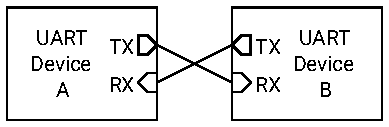
\includegraphics{figures/uart-connection-diagram.pdf}
	\caption{UART Connection Diagram}
	\label{fig:uart-connection-diagram}
\end{figure}



\subsection{Generalized UART Transmission Process}

\begin{figure}[htpb]
	\begin{tikztimingtable}[timing/font=\rmfamily, timing/d/text/.append style={font=\rmfamily}, xscale=3.5, yscale=2, timing/slope=0.2, timing/dslope=0.2, timing/d/background/.style={fill=white},
		timing/metachar={{K}[2]{#1H !{++(-.5\xunit + 0.5*\slope\xunit, -.5\yunit)} N[rectangle,scale=.6]{#2} !{++(.5\xunit - 0.5*\slope\xunit, +.5\yunit)}}},
		timing/metachar={{J}[2]{#1L !{++(-.5\xunit + 0.5*\slope\xunit, +.5\yunit)} N[rectangle,scale=.6]{#2} !{++(.5\xunit - 0.5*\slope\xunit, -.5\yunit)}}},]
		TX or RX & K{IDLE} J{START} D{D0} D{D1} D{D2} D{D3} D{D4} D{D5} D{D6} D{D7} D{\textrm{[P]}} K{STOP} K{IDLE} \\
	\end{tikztimingtable}
	\caption{UART Data Frame Timing Diagram}
	\label{fig:uart-timing-diagram}
\end{figure}

Each UART wire is unidirectional, with the TX pin of the transmitting device driving the logic level of the wire and the RX pin of the receiving device reading the level of the pin. The only distinction between the two wires is the direction that data travels, and as such, this section will only depict one wire.

When no UART transmission is occurring, the UART wire is idle, and the TX pin drives the UART wire high. To start a transmission, the TX pin transmits a start bit by driving the wire low for $T_B = 1 / \textrm{baud}$ seconds. It then begins transmitting each data bit, LSB-first, every $T_B$ seconds until all 8 bits have been transmitted. Then, it optionally transmits a parity bit, which helps detect transmission errors. Finally, it transmits a stop bit by driving the wire high for $T_B$ seconds. After that point, it may begin another transmission by sending another start bit, or it can let the wire be idle.

Figure \ref{fig:uart-timing-diagram} shows a timing diagram for the UART transmission process. Note that the parity bit [P] is optional.



\subsection{UART Baud Generation}

Both devices communicating over the UART must agree on the baud rate, or the number of bits transmitted per second. In the absence of a clock wire, the UART uses the baud rate to sample the RX wire every $T_B = 1/\ \textrm{baud}$ seconds, recording the logic levels in sequence. The transmitter must send bits at that same rate. Any significant deviation of the baud rate can result in bit errors.

The UART uses 16× oversampling for improved noise immunity and accurate bit detection. The baud rate for the \peripheral{UARTx} peripheral is configured through the 12-bit \register{UARTxBR} register:

\begin{equation*}
	\textrm{UART baud} = \frac{f_\textrm{SMCLK}}{16 \times (\bitfield{BR} + 1)}
\end{equation*}

For example, with SMCLK running at 48 MHz:
\begin{itemize}
	\item \bitfield{BR} = 25 gives 115,200 baud
	\item \bitfield{BR} = 51 gives 57,600 baud
	\item \bitfield{BR} = 103 gives 28,800 baud
\end{itemize}



\subsection{Parity Bit}

A UART frame has an optional parity bit after the last data bit and before the stop bit. The purpose of the parity bit is to verify that the data received is indeed the data that was transmitted. If the received parity bit does not match the expected parity bit, then the receiver knows that the received data has been corrupted.

If the parity bit is enabled with \bitfield{UPEN}, the transmitter calculates the parity of the byte to transmit by taking the exclusive OR of all 8 bits in the transmitted byte, the result of which is then put through a final exclusive OR gate with the parity select bit \bitfield{UPSEL}:
\begin{equation*}
p = b_7 \oplus b_6 \oplus \cdots \oplus b_1 \oplus b_0 \oplus \bitfield{UPSEL}
\end{equation*}
When \bitfield{UPSEL} is 0, the parity is said to be ``even'', and when it is 1, ``odd''. This operation is functionally counting how many bits are 1s in the transmitted byte. When even parity is selected, the parity bit is 0 when the number of 1s is even and 1 when the number of 1s is odd. That result is inverted when odd parity is selected.

On the receiver end, the parity bit is capable of detecting a single bit error in the transmission. That is, if one of the eight data bits (or the parity bit itself) is incorrectly received, then the parity error flag \bitfield{UPEF} will detect a bit error. However, if two bits are incorrectly received, then the parity error flag will not detect the bit error. Note that if the number of bit errors is an odd number, the parity error flag will detect the error, but will not when the number of bit errors is even.

If a parity bit is enabled on the transmitter side, it must also be enabled on the receiver side with \bitfield{UPEN}.



\subsection{Transmit Buffer Register Queue}

Writing to the UART transmit buffer register \register{UARTxTX} queues up the byte written to it as the next frame to transmit. If a transmission is not currently ongoing, the \peripheral{UARTx} peripheral immediately begins transmitting the byte written to \register{UARTxTX}, and \bitfield{TEIF} is set immediately. If a transfer is currently ongoing, the \peripheral{UARTx} peripheral waits for the current frame to finish transferring. As soon as it finishes, the \peripheral{UARTx} peripheral begins transmitting the new frame written to \register{UARTxTX} and sets \bitfield{TEIF}.

The TX queue allows the \peripheral{UARTx} peripheral to constantly transfer data without any dead time in between frames, ensuring maximum transfer speed. However, the user must take care not to overflow the queue, which happens if the \register{UARTxTX} is written two or more times during a single frame transfer. Queue overflows can be prevented by waiting for the \bitfield{TEIF} flag to be 1 or \bitfield{TXBF} to be 0 before writing to \register{UARTxTX}.



\subsection{Flags and Interrupts}

The \peripheral{UARTx} peripheral has five status flags and three interrupt flags in the \register{UARTxSR} register. If the corresponding interrupts are enabled in the \register{UARTxCR} register and the \peripheral{UARTx} ISR is not masked, then the three interrupt flags will generate an interrupt whenever they are equal to 1. Any and all interrupt flags must be cleared before the \peripheral{UARTx} ISR returns, else the ISR will mistakenly re-execute immediately upon the prior return.

The \register{UARTxSR} and \register{UARTxRX} registers are latched on the falling edge of the memory enable signal for improved noise immunity during reads.

The UART receiver busy flag \bitfield{RXBF} shows when the \peripheral{UARTx} peripheral is currently receiving a byte of data when it is 1. Likewise, \bitfield{TXBF} indicates that a transmission is ongoing or pending when 1.

The UART framing error flag \bitfield{FEF} indicates that a framing error occurred on the last reception when it is a 1. A framing error typically occurs if the UART transmitter settings do not match the receiver settings, such as baud rate, number of bits to transmit, or the presence/absence of a parity bit. Specifically, a framing error is detected if the receiver does not detect a high level at the expected stop bit time. If \bitfield{FEF} is a 1 after a reception, that reception must be treated as unrecoverable, corrupted data. \bitfield{FEF} is cleared when the \register{UARTxRX} register is read.

The UART parity error flag \bitfield{PEF} indicates that a parity error occurred on the last reception when it is a 1. A parity error can only happen if the parity bit is enabled by setting \bitfield{PEN} to 1. A parity error occurs when the parity bit appended to the received data byte does not match the expected value calculated from the received data. If \bitfield{PEF} is a 1 after a reception, that reception must be treated as corrupted data. \bitfield{PEF} is cleared when the \register{UARTxRX} register is read.

The UART receive data overflow flag \bitfield{OVF} indicates that the user did not read the \register{UARTxRX} register in time before another byte of data was received by the \peripheral{UARTx} peripheral when it is a 1. In this case, the previous received data has been lost and must be treated as incomplete. \bitfield{OVF} is cleared when the \register{UARTxRX} register is read.

The UART receive complete interrupt flag \bitfield{RCIF} is set to 1 immediately when the \peripheral{UARTx} peripheral finishes receiving a frame of data from the transmitter. The new data byte becomes available in the \register{UARTxRX} register as soon as \bitfield{RCIF} is set. This is also the moment that \bitfield{FEF}, \bitfield{PEF}, and \bitfield{OVF} flags will be updated, if the proper conditions are met. \bitfield{RCIF} is cleared when the \register{UARTxRX} register is read or by writing a 1 to this bit in \register{UARTxSR}.

The UART transmit register empty interrupt flag \bitfield{TEIF} is set the moment the UART TX buffer register \register{UARTxTX} becomes empty (i.e., is ready to queue up the next byte to transmit). If a frame is not currently being transmitted, the flag is set immediately when a new byte is written to \register{UARTxTX}. If a frame is currently being transmitted, it is set as soon as the current transfer is completed, whereupon the value in the \register{UARTxTX} register begins to be transmitted. Write a 1 to this bit in \register{UARTxSR} to clear \bitfield{TEIF}.

The UART transmit complete interrupt flag \bitfield{TCIF} is set the moment the UART transmission completes (all bits sent) and the transmitter becomes idle. Write a 1 to this bit in \register{UARTxSR} to clear \bitfield{TCIF}.



\subsection{Transmit Procedure}

To transmit a byte of data via the UART, first initialize the \peripheral{UARTx} peripheral by configuring the \register{UARTxCR} register and setting the baud rate with the \register{UARTxBR} register. Of note, the UART enable bit \bitfield{EN} must be a 1 to activate the UART. When \bitfield{EN} is 0, the UART peripheral is held in reset state. The GPIO pin multiplexed with \pin{TXx} must be set to secondary/peripheral mode in the corresponding \register{PxSEL} register.

To transmit a byte of data over the UART, first clear the status register by reading it and discarding its value. Then, wait until the UART is not transmitting (when \bitfield{TXBF} is 0) or the UART TX buffer is empty (when \bitfield{TEIF} is 1). Next, write the byte to transmit to the \register{UARTxTX} register. The byte will be finished transmitting once \bitfield{TXBF} is 0.

A simplified procedure for transmitting a byte over the UART is shown in Listing \ref{lst:uart-tx}.

\begin{lstlisting}[style=customC, label=lst:uart-tx, caption={Example Function for UART Transmissions}]
/** Includes **/
#include <MemoryMap.h>

/** Function Definitions **/
void uartx_putc(char tx_data)
{
	// Wait for the transmitter to finish any previous transmissions
	while (UARTxSR & TXBF) { }
	
	// Send the new data byte
	UARTxTX = tx_data;
}
\end{lstlisting}



\subsection{Receive Procedure}

To receive a byte of data via the UART, first initialize the \peripheral{UARTx} peripheral by configuring the \register{UARTxCR} register and setting the baud rate with the \register{UARTxBR} register. Of note, the UART enable bit \bitfield{EN} must be a 1 to activate the UART. The GPIO pin multiplexed with \pin{RXx} must be set to secondary/peripheral mode in the corresponding \register{PxSEL} register.

Once done setting up the UART, wait for the UART receive complete interrupt flag \bitfield{RCIF} to be 1. Then, read the received byte contained in the \register{UARTxRX} register. Reading \register{UARTxRX} automatically clears the \bitfield{RCIF}, \bitfield{FEF}, \bitfield{PEF}, and \bitfield{OVF} flags.

A simplified procedure for receiving a byte over the UART is shown in Listing \ref{lst:uart-rx}.

\begin{lstlisting}[style=customC, label=lst:uart-rx, caption={Example Function for UART Receptions}]
/** Includes **/
#include <MemoryMap.h>

/** Function Definitions **/
char uartx_getc()
{
	// Wait for the UART to receive a new character
	while ((UARTxSR & RCIF) == 0) { }
	
	// Return the new character that is in the receive buffer register
	return UARTxRX;
}
\end{lstlisting}



\subsection{\peripheral{UART0} Boot Behavior}

When booting in Forth interpreter mode, the \peripheral{UART0} peripheral provides an interactive command processor with an external device, such as computer with a USB to UART device attached. When the MCU is powered up or reset and the \pin{BOOT} pin is low, the Forth interpreter will launch over \peripheral{UART0}, which can be used to program or debug the MCU.

Section \ref{s:startup} elaborates on the power up and reset behavior of the MCU.
